\documentclass[twocolumn]{article}

\newcommand{\Title}{Caldera-like features located over the Panikkar Seamount and adjacent regions in the Laxmi Basin, Eastern Arabian Sea}
\newcommand{\Journal}{Journal of Earth System Science}
\newcommand{\Author}{J. John Savio, V. Yatheesh, et al.}

\newcommand{\AuthorAffil}{
	{\large
		J. John Savio$^{1,2}$
		V. Yatheesh$^{1,*}$
		R. Sheldon$^{1}$
		M. Kallathian$^{1}$
		Pratima Kessarkar$^{1}$}\\
	{\large
		Kuldeep Kumar$^{1}$
		P. Mahesh$^{1}$
		Subhashree Mishra$^{1}$
		Swati Verma$^{1}$
	}
	\\[0.4cm]
	{\small $^1$ CSIR -  National Institute of Oceanography, Dona Paula, Goa -  403 004, India}
	\\
	{\small $^2$ School of Earth, Ocean and Atmospheric Sciences, Goa University, Taleigao Plateau, Goa -  403 206, India}
	\\
	{\small $^*$ Corresponding author e-mail: yatheesh@nio.org}
}
\newcommand{\DOI}{doi:\href{https://doi.org/10.xxxx/jess/xxxxxx}{10.xxxx/jess/xxxxxx}}
\newcommand*{\doi}[1]{doi:\href{http://dx.doi.org/#1}{#1}} %% To give hyperlink to DOI's

\usepackage[left=0.7in,right=0.7in,top=0.9in,bottom=0.8in]{geometry}
\setlength{\columnsep}{2\columnsep}
\usepackage[utf8]{inputenc}
\usepackage{timet}
\usepackage{amsmath}
\usepackage{ragged2e}
\usepackage{graphicx}
\usepackage[round]{natbib}
\hbadness=99999
%%\usepackage{fixltx2e}
\usepackage{url}
\usepackage[pdftex,colorlinks=true]{hyperref}
\hypersetup{
	allcolors=blue,
	pdftitle={\Title},
	pdfauthor={\Author},
}
\usepackage{fancyhdr}
\pagestyle{fancy}
\usepackage{caption}
\fancyhf{}
\lhead{
	\fontsize{9pt}{12pt}\selectfont
	\Author{}, 2021, \DOI{}
}
\rhead{\fontsize{9pt}{12pt}\selectfont \thepage}
\renewcommand{\headrulewidth}{0pt}

\begin{document}
\title{\Title}
\author{\AuthorAffil}
\date{
\normalsize
Manuscipt Received - xx June 2021; Revised - xx October 2021; Accepted - 05 November 2021
\\[0.4cm] 
\justifying{
This is a pre-copyedited, author-produced version of an article accepted for publication in \textit{\Journal{}} following peer review. The version of record "\textit{John Savio, J., Yatheesh, V., Sheldon, R., Kallathian, M., Kessarkar, P., Kumar, K., Mahesh, P., Mishra, S., \&  Verma, S., 2021. \Title{}, \Journal{},}\ " is available online at: \DOI{}
}}
\maketitle

\begin{abstract}
The Laxmi Basin, which is believed to have been formed by the divergence between India and the Laxmi Ridge, contains a seamount chain consisting of the Raman Seamount, Panikkar Seamount and the Wadia Guyot in its axial region. Some authors considered that these seamounts are underlain by stretched continental crust, while others attributed the genesis of these seamounts to an anomalous episode of volcanism resulting from the interaction of the R\'eunion hotspot with the extinct spreading centre. In absence of any direct evidences to these contradicting views, we carried out a detailed multibeam bathymetry survey over a selected sector of this seamount chain and collected a fresh set of high-resolution bathymetry data. Our analysis of this bathymetry data reveals the presence of six semicircular scarp faces enclosing nearly flat seafloor over the Panikkar Seamount, with their morphology resembling with the shape of volcanic calderas. Based on the presence of these caldera-like features, in conjunction with the constraints of plate tectonic framework of this region, we corroborate the volcanic origin for the seamount chain located in the axial part of the Laxmi Basin.
\\[0.6cm]
\textbf{Keywords:}
Volcanic caldera; Laxmi Basin; Panikkar Seamount; bathymetry; morphology.
\end{abstract}


\section{Introduction}
The deep ocean basin existing between the Laxmi Ridge in the west and the Indian continental margin in the east represents the Laxmi Basin (Figures \ref{fig:studyarea} \& \ref{fig:studyarea2}). Although the researchers broadly agree that the Laxmi Basin was formed by divergence, difference in opinion exists about the nature of crust underlying this basin. Some researchers \citep{Naini1982,Kolla1990,Todal1998,Krishna2006,Nemcok2017,Geoffroy2020} consider this basin to have been formed only by continental rifting resulting in thinned continental crust, while others \citep{Biswas1988,Bhattacharya1994a,Talwani1998,Bernard2000,Yatheesh2007,Corfield2010,Eagles2013,Siawal2014,Bhattacharya2015,Misra2015,Ramana2015} consider this basin to have been formed by continental rifting followed by seafloor spreading resulting in the formation of the oceanic crust. The inference on continental origin of the Laxmi Basin is mainly based on the semi-continental crustal thickness and lack of identifiable seafloor spreading type magnetic anomalies, while the oceanic origin is inferred based on the symmetric magnetic anomalies that can be explained in terms of juxtaposed normal and reversely magnetized oceanic crustal blocks, hyperbolic reflection pattern in the multi-channel seismic reflection sections, and the presence of Seaward Dipping Reflectors (SDRs) landward of the Laxmi Ridge and seaward of the western continental slope of India.
The axial part of the Laxmi Basin is characterized by the presence of three isolated seamounts, referred to as the Raman Seamount, Panikkar Seamount and Wadia Guyot \citep{Bhattacharya1994b}, from the north to south (Figures \ref{fig:studyarea} \& \ref{fig:studyarea2}). These seamounts, together forming an axial seamount chain in the Laxmi Basin \citep{Bhattacharya1994b}, situates on an ~ 360 km long, NNW-SSE striking ridge buried under the sediments (Figures \ref{fig:studyarea} \& \ref{fig:studyarea2}), referred to as the Panikkar Ridge \citep{Gopala_Rao1992}. The supporters of continental origin hypothesis for the formation of the Laxmi Basin interpreted the Panikkar Ridge to\begin{figure*}[!htb]
	\centering
	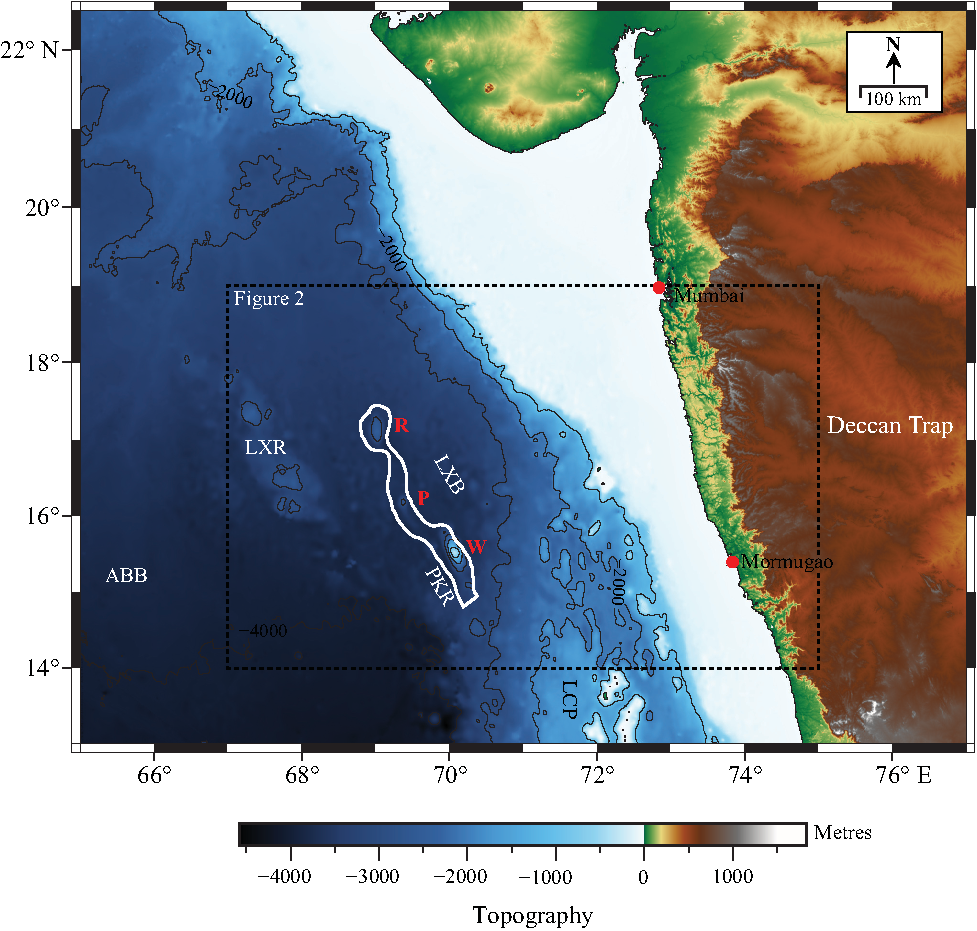
\includegraphics[width=0.85\linewidth]{studyarea-bathy.pdf}
	\caption{
	Topographic map of the northwestern continental margin of India and the adjoining deep oceans basins as depicted by the GEBCO 2021 global terrain model for ocean and land \citep{GEBCO_Compilation_Group2021}, showing the locations of the Panikkar Ridge (shown as thick white line) and the axial seamount chain in the Laxmi Basin. Thin black lines are selected (1000 m., 2000 m., 3000 m., and 4000 m.) bathymetry contours from GEBCO 2021 data set. The box shown with thick dashed black lines represents the boundary of the tectonic map shown in Figure 2. LXR: Laxmi Ridge; LXB: Laxmi Basin; ABB: Arabian Basin; PKR: Panikkar Ridge; LCP: Laccadive Plateau. R: Raman Seamount; P: Panikkar Seamount; W: Wadia Guyot
	}
	\label{fig:studyarea}
\end{figure*} represent a structural feature of less altered stretched continental crust \citep{Krishna2006}, or an isolated continental block \citep{Geoffroy2020}. \cite{Krishna2006} further considered that the Raman Seamount, Panikkar Seamount and Wadia Guyot represent the isolated highs of the Panikkar Ridge elevated above the seafloor, implying a continental origin for these seamounts. In contrary to this, the supporters of oceanic crust hypothesis for the formation of the Laxmi Basin inferred that the Panikkar Ridge represents the extinct spreading centre in the Laxmi Basin \citep{Bhattacharya1994a,Bhattacharya1994b}, where two-limbed seafloor spreading initiated at around 67.6 Ma and ceased at ~56.4 Ma, as interpreted from the identified magnetic anomaly sequence C30n-C25r-C30n \citep{Bhattacharya2015,Yatheesh2020}. Further, those studies attributed the genesis of the Raman-Panikkar-Wadia seamount chain located over the Panikkar Ridge to an anomalous episode of volcanism resulting from the interaction of the R\'eunion hotspot with the spreading centre in the Laxmi Basin. These seamounts are considered to have been emplaced at around 62.5 Ma \citep{Bhattacharya2015,Yatheesh2020}, coeval with the emplacement of Ghatkopar-Powai tholeiites on the Indian mainland \citep{Pande2017}. However, any direct evidences from this seamount chain to represent their genesis in terms of volcanic eruptions is still awaited. Towards this, we carried out a multibeam bathymetry survey over a selected sector of this seamount chain to
\begin{figure*}[!htb]
	\centering
	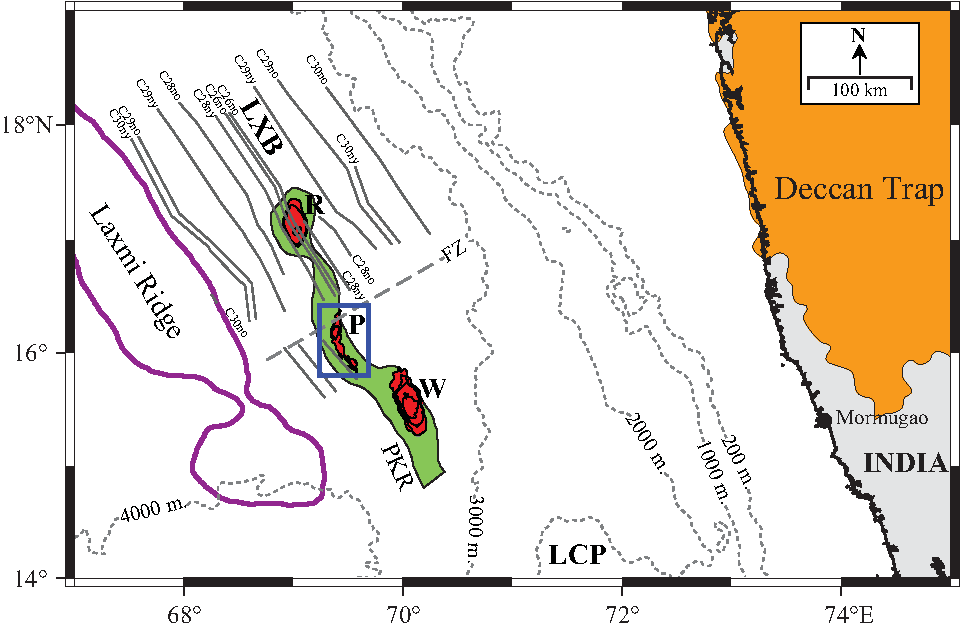
\includegraphics[width=0.8\linewidth]{tectonic-framework.pdf}
	\caption{
		Generalized tectonic map of the northwestern continental margin of India and the adjoining deep ocean basins. The blue coloured box represents the study area. Grey coloured thin dotted lines represent the selected (200 m., 1000 m., 2000 m., 3000 m., and 4000 m.) bathymetry contours. Grey coloured continuous lines represent the inferred magnetic lineations in the Laxmi Basin  \citep{Bhattacharya2015} and the solid red coloured patches in the axial part of the Laxmi Basin represent the extent of the seamount chain \citep{Bhattacharya1994b} consisting of the Raman Seamount (R), Panikkar Seamount (P) and the Wadia Guyot (W). The green-coloured region represents the extent of the Panikkar Ridge (PKR).  Other details are as in Figure \ref{fig:studyarea}.
	}
	\label{fig:studyarea2}
\end{figure*}
understand the detailed seafloor morphology of this anomalous feature. In this paper, we present the preliminary morphotectonic information derived from the analysis of this fresh set of recently acquired high-resolution multibeam bathymetry data.
%%%%%%%%%%%%%%%%%%%%%%%%%%%%%%%%%%%%%%%%%%%%%%%%%%%%%%%%%%%%%%%%%%%%%%%%%%%%%%
\section{Data and Methodology}
A multidisciplinary scientific expedition was conducted onboard \textit{RV Sindhu Sadhana}, by the CSIR – National Institute of Oceanography, Goa, India, during 28\textsuperscript{th} August to 10\textsuperscript{th} September 2020. As a part of this expedition, multibeam bathymetry data were collected over selected sectors in the axial part of the Laxmi Basin, where the Raman-Panikkar-Wadia seamount chain is located. The multibeam bathymetry data was collected using Teledyne-Atlas multibeam echo sounders, operated at a frequency of 15 kHz. These data were corrected for variation of sound velocity in sea water by collecting sound velocity profiles in real time. The PDS software was used to process the data, first by removing erroneous values and then applying the most suitable qualitative filters. Using this data, a bathymetric grid of 100 m spatial resolution was generated and the bathymetric maps were plotted using the Generic Mapping Tools software \citep{Wessel2019}.
%%%%%%%%%%%%%%%%%%%%%%%%%%%%%%%%%%%%%%%%%%%%%%%%%%%%%%%%%%%%%%%%%%%%%%%%%%%%%
\begin{figure*}[!htb]
	\centering
	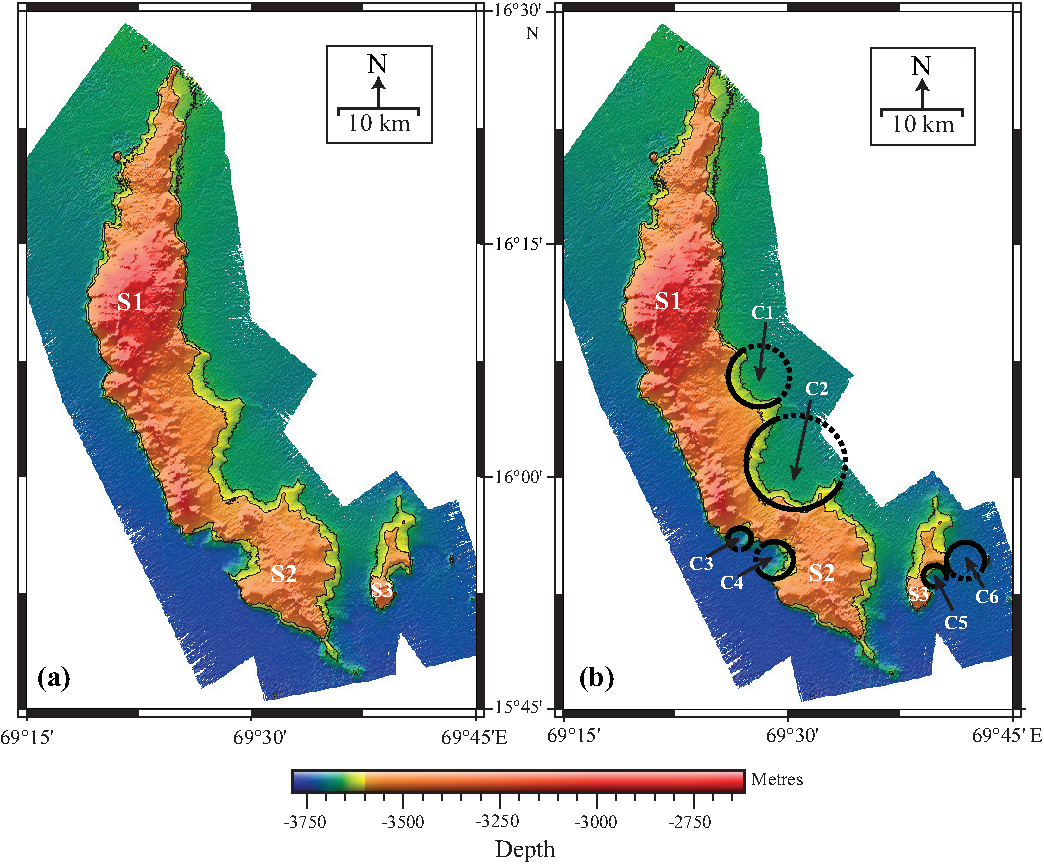
\includegraphics[width=\textwidth]{panikkar-seamount.pdf}
	\caption{
		Colour-coded bathymetric map of the Panikkar Seamount and the adjacent regions, showing (a) the morphology of the seafloor and (b) the interpreted caldera-like features. The thin black lines represent selected (3600 m. and 3650 m.) isobaths. S1, S2 and S3 represent the Segment-1, Segment-2 and Segment-3 of the Panikkar Seamount. The labels C1 through C6 represent the locations of inferred caldera-like features. The thick black circles represent the postulated extent of rims of these inferred calderas as seen from the bathymetry data (continuous semi-circles) and as considered to have buried under the sediments (dotted semi-circles).
	}
	\label{panikkar}
\end{figure*}
%%%%%%%%%%%%%%%%%%%%%%%%%%%%%%%%%%%%%%%%%%%%%%%%%%%%%%%%%%%%%%%%%%%%%%%%%%%%%
\section{Preliminary results and discussion}
We present high-resolution multibeam bathymetry data as a colour-coded two-dimensional (Figures \ref{panikkar}a\&b) and three-dimensional (Figures \ref{calderas}a-c) images over a segment of the Laxmi Basin Seamount chain, i.e., over the Panikkar Seamount and the adjoining regions. The multibeam bathymetric map (Figure \ref{panikkar}a) clearly depicts the presence of three bathymetric highs, together forming an arcuate shape. Among these, the two larger features with major peaks sitting on a single base defined by 3600 m. isobath, represent the Panikkar Seamount discovered by \cite{Bhattacharya1994b}. The third bathymetric high identified in the present study also appears to form a part of this anomalous feature, and therefore, Panikkar Seamount can be considered to consists of three segments. For the ease of reference, in this paper, we refer these segments as Segment-1 (S1), Segment-2 (S2) and Segment-3 (S3) of the Panikkar Seamount, from northwest to southeast, respectively (Figure \ref{panikkar}a). Among these, the Segment-1 (S1) represents the largest feature, whose western side is characterized by a sharp boundary defined by the 3650 m. and 3600 m. isobaths. In the eastern side of this segment, north of 16°09’N, the bathymetric high shows similar sharp drop in the depth as in the case of western limit, however, towards south, this feature shows a relatively gentle topography. Similarly, the Segment-2 (S2) is associated with a sharp boundary in the southwestern side and a relatively gentle topography on its eastern side. However, the bathymetric map of the regions adjacent to these two segments, Segment-1 and Segment-2, clearly depicts the presence of isolated, characteristic semi-circular, scarp faces / embayments with a moderately steep slope that are dipping to a nearly flat seafloor region away from the crest of the seamount, in the southwestern as well as eastern sides of these anomalous bathymetric features (Figure \ref{panikkar}a). Similarly, the Segment-3, which is separated from Segment-2 by a relatively deeper seafloor, is also characterized by the presence of two smaller semi-circular bathymetric features (Figure \ref{panikkar}a). Morphologically, such rim-like features enclosing a region of nearly flat seafloor associated with all the three segments of the Panikkar Ridge are very interesting, since this geometry closely resembles with the shape of volcanic caldera structures associated with the submarine volcanic events. Such volcanic calderas generally form due to the collapse or subsidence into the top of a magma chamber \citep{Cole2005}. \cite{Bijesh2021} has recently reported the presence of an extinct giant volcanic caldera in the Arabian Sea, southwest of the Laccadive Plateau, based on the presence of a nearly elliptical bathymetry high complex, known as the Sagar Kanya Bathymetric High Complex, enclosing a nearly flat seafloor region.
\begin{minipage}{\linewidth}% to keep image and caption on one page
	\vspace{7.5mm} %5mm vertical space
	\makebox[\linewidth]{%        to center the image
		\noindent\includegraphics[width=1.09\linewidth,keepaspectratio]{panikkar-caldera.pdf}}
	\captionof{figure}{ Colour-coded three-dimensional bathymetry maps representing postulated calderas (a) C1 and C2; (b) C3 and C4; and (c) C5 and C6. Other details are as in Figure \ref{panikkar}.}\label{calderas}
	\vspace{4mm} %5mm vertical space
\end{minipage}

From the colour-coded two-dimensional bathymetric image (Figure \ref{panikkar}a, b), we identify six semi-circular scarp faces, labeled as C1, C2, C3, C4, C5 and C6, having diameters 6.7 km., 11.7 km., 2.3 km., 4.5 km., 2.5 km., and 4.0 km., respectively, and present their morphology in three-dimensional perspective (Figures \ref{calderas} a-c). It is important to note that almost all these scarp faces are semi-circular in nature, but theoretically, all the volcanic calderas should be associated with circular rim structures. To examine this, we referred the published literature depicting the morphology of various known volcanic calderas, such as  the Santorini Caldera \citep{Nomikou2012}, Nikko Submarine Volcanic Caldera \citep{Global_Volcanism_Program1990}, the Brothers Seamount Caldera \citep{Stagpoole2016}, Henderson Seamount Caldera \citep{Taylor1980}, and the Sagar Kanya Volcanic Caldera \citep{Bijesh2021}. Interestingly, none of these volcanic calderas are associated with complete circular rim structures all over 360°, as seen in the bathymetry data, and the absence of rim structure at parts of these calderas have been interpreted to represent a morphological configuration of buried rim structure, associated with the asymmetrical subsidence resulted by tilting of the magma chamber \citep{Kennedy2004}. We believe, this explanation reasonably holds good to explain the semi-circular nature of the postulated volcanic calderas adjacent to the Panikkar Seamount; the segments of the rim structure missing from the seafloor image might represent buried rim structure associated with asymmetric subsidence as in the case of the above volcanic calderas and the observed dipping of seafloor containing the rim structure away from the crest of the seamount towards deeper region further support this asymmetric subsidence and tilting of magma chamber.

It may be noted that the inferred caldera-like features are concentrated south of 16° 08’N latitude on the Panikkar Seamount, while the northern part of this seamount is devoid of such prominent features. In the north, the Segment S-1 contains multiple peaks on a single base and the least depth over the largest of these peaks (near 16°13'N) is about 2618 m., which is much higher from the surrounding seafloor than the other two segments, suggesting multiple phases of volcanism over the Segment S-1 of the Panikkar Seamount. As in the case of region south of 16° 08’N latitude, volcanic caldera-like features might have been formed in this norther region also, however, the later phases of volcanism occurred in the northernmost part of the Panikkar Seamount might have obliterated the morphological features representing caldera-like feature formed as a result of the early phases of volcanism.   
%%%%%%%%%%%%%%%%%%%%%%%%%%%%%%%%%%%%%%%%%%%%%%%%%%%%%%%%%%%%%%%%%%%%%%%%%%%%%%%

\section{Summary and Conclusion}

The updated bathymetric map of the Panikkar Seamount and the adjacent regions depicts the presence of three segments of bathymetric highs, of which two larger features (Segment-1 and Segment-2) are sitting on a single base defined by 3600 m. isobath and the third one (Segment-3) is separated from Segment-2 by a relatively deeper seafloor. These regions are associated with six characteristic semi-circular scarp faces enclosing nearly flat seafloor, deepening away from the crest of the major peak of the bathymetric highs of all the segments. We interpret these features to represent volcanic calderas associated with the submarine volcanic events. Considering the presence of these volcanic calderas over the Panikkar Seamount and the adjacent regions, in conjunction with the published information on the presence of an extinct spreading centre under the influence of R\'eunion hotspot, we attribute the genesis of seamount chain in the Laxmi Basin to the R\'eunion hotspot volcanism during the waning stage of seafloor spreading in the Laxmi Basin. Therefore, based on the analysis of our recently collected multibeam bathymetry data, we corroborate volcanic origin for the seamount chain in the axial part of the Laxmi Basin in contrary to the concept of underlying continental crust. However, a detailed geochronological investigation by collecting the rock samples from this region needs to be carried out for providing age constraint for this inferred episode of volcanism responsible for the formation of the Panikkar Seamount.

%%%%%%%%%%%%%%%%%%%%%%%%%%%%%%%%%%%%%%%%%%%%%%%%%%%%%%%%%%%%%%%%%%%%%%%%%%%%%%%

\section*{Acknowledgments}

The authors are grateful to Prof. Sunil Kumar Singh, Director, CSIR-National Institute of Oceanography (CSIR-NIO), Goa, India, for providing ship time and granting permission to publish this work. This study forms a part of PhD work of JJS at Goa University. JJS thank Council of Scientific \& Industrial Research (CSIR), New Delhi, India, for the financial support under Junior Research Fellowship (Grant No. 31/026(0321)/2019-EMR-I). The cooperation and support received from the Captain and his operational team onboard \textit{RV Sindhu Sadhana} during the expedition SSD-073 are acknowledged. We thank Dr. V.J. Loveson, Head, Geological Oceanography Division for useful discussions, and Mr. S. Gautham for the help extended in processing the bathymetry data. We are grateful to an anonymous reviewer for his constructive review and valuable suggestions that improved our manuscript, and to Dr. N.V. Chalapathi Rao for editorial handling. All figures were drafted with the GMT software  \citep{Wessel2019}. This is NIO contribution xxxx.


%%%%%%%%%%%%%%%%%%%%%%%%%%%%%%%%%%%%%%%%%%%%%%%%%%%%%%%%%%%%%%%%%%%%%%%%%%%%%%%

\section*{Author statement}

J. John Savio: Conceptualized the idea, acquisition and processing of the data, preparation of first draft of the manuscript; V. Yatheesh: Conceptualized the idea, interpretation, correction of the manuscript; R. Sheldon: Data acquisition and quality check; M. Kallathian: Data acquisition and quality check; Pratima Kessarkar: Data acquisition; Kuldeep Kumar: Data acquisition; P. Mahesh: Data acquisition; Subhashree Mishra: Data acquisition; Swati Verma: Data acquisition. All authors contributed to the correction and finalization of the manuscript.


%%%%%%%%%%%%%%%%%%%%%%%%%%%%%%%%%%%%%%%%%%%%%%%%%%%%%%%%%%%%%%%%%%%%%%%%%%%%%%%

\bibliographystyle{gji-doi-link}
\bibliography{references}
\appendix


\end{document}

